\documentclass[a4paper, 11pt, titlepage]{article}
\usepackage{fancyhdr}
\usepackage{graphicx}
\usepackage{imakeidx}
\usepackage{makeidx}
\usepackage{mathtools}
\usepackage[spanish]{babel}
\usepackage{eurosym}
\usepackage{hyperref}
\usepackage{amssymb}
\usepackage{listings}
\usepackage{xcolor}

% \setcounter{secnumdepth}{5}
% \setcounter{tocdepth}{5}

\title{Inteligencia artifical}
\author{Francisco Javier Balón Aguilar}

\begin{document}

\maketitle
\renewcommand{\contentsname}{Índice}
\tableofcontents
\newpage

\section{Contextualización}

    La inteligencia artifical puede definirse como una rama de la computación dedicada al
    desarrollo de agentes inteligentes no vivos por medio de las técnicas de la computación 
    y la programación.

    \paragraph{Etapa anterior al siglo XX} Las bases en las que se apoya el desarrollo de la inteligencia 
    artificial son anteriores al siglo XX, concretamente podemos ver su origen en la antigua Grecia.

    Aristóteles hacia el año 300 a.C. ya definió, en sus estudios, lo que conocemos como 
    \textbf{silogismos}\footnote{
        Un silogismo es un conjunto estructurado de reglas que describen una parte del conocimiento, 
        a partir de las cuales se pueden establecer conclusiones racionales en base a unas 
        premisas dadas.
    }. Posteriormente, hacia el año 1.315, Ramón Llull, basándose en otra herramienta astrológica 
    árabe, para combinar conceptos mecánicamente. Esta máquina estaba formada por tres discos 
    giratorios concéntricos que albergaban regiones en las que se ubicaban determinadas categorías 
    del pensamiento; es decir, girando estos discos se formaban nuevas teorías (véase imagen 
    \ref{arsmagna}).

    \begin{figure}[htp]
        \centering
        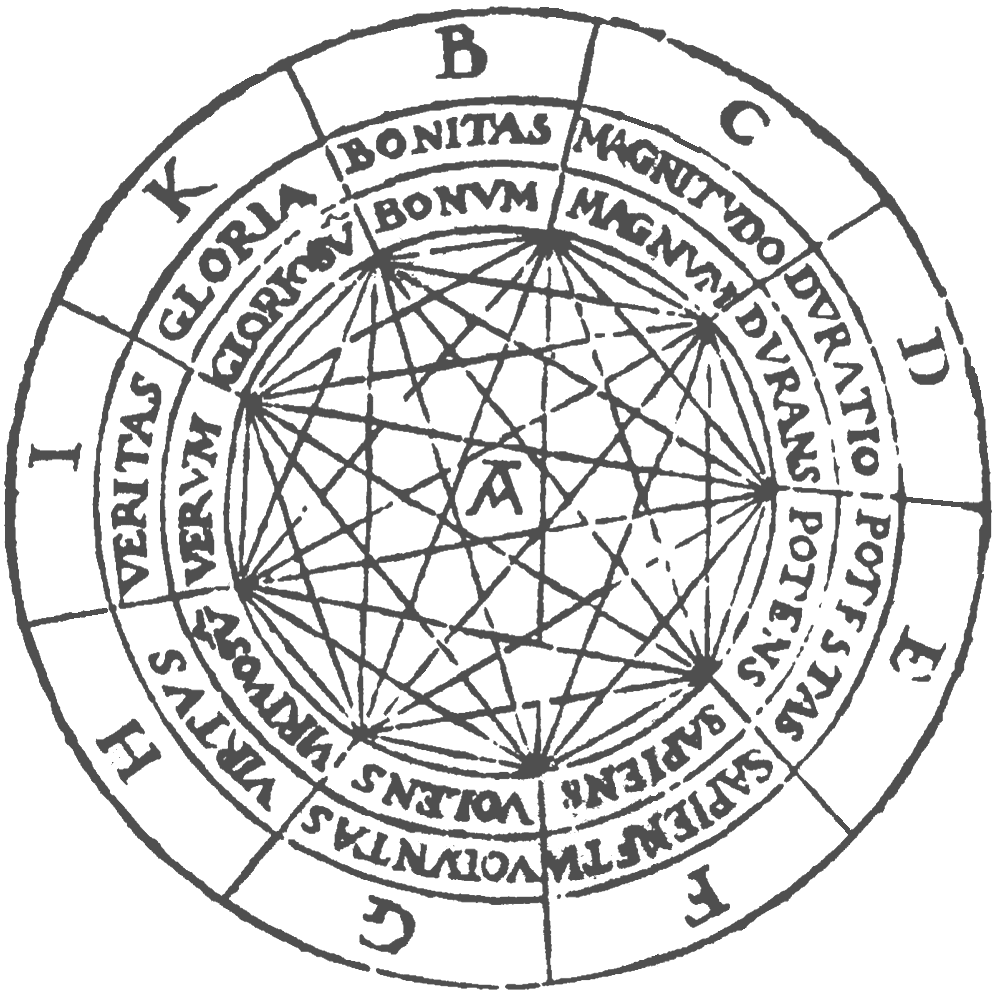
\includegraphics[width=0.4\textwidth]{resources/arsmagna.png}
        \caption{Esquema de la máquina Ars Magna, de Ramón Llull.}
        \label{arsmagna}
    \end{figure}

    En el año 1.842, Charles Babbage es considerado el padre de la informática por la creación de la 
    primera calculadora mecánica programable (véase imagen \ref{maquinabaggage}), introduciendo las bases 
    de la computación.

    \begin{figure}[htp]
        \centering
        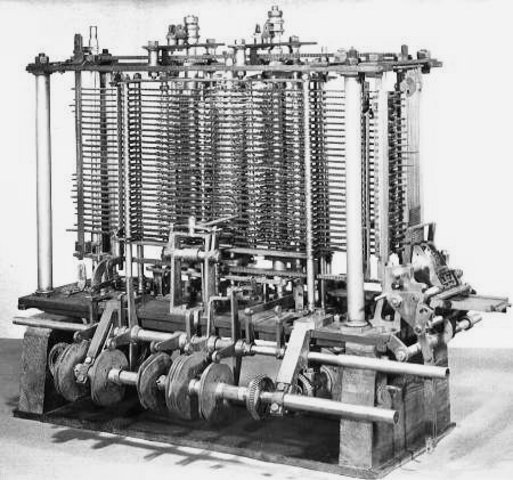
\includegraphics[width=0.6\textwidth]{resources/maquinababbage.jpg}
        \caption{Máquina analítica de Babbage.}
        \label{maquinabaggage}
    \end{figure}

    Unos años más tarde, en 1.847, George Bool con su llamada lógica booleana o proposicional, mientras 
    investigaba las leyes fundamentales sobre las que basa el razonamiento humano y su expresión matemática, 
    añadió complejidad a la lógica de Aristóteles. Basándose en estos estudios, en 1.879, Gottlob Frege extiende 
    la lógica booleana creando la lógica de Primer Orden, utilizada hasta nuestros días y con una escalabilidad 
    de expresión mayor que la lógica booleana.

    \paragraph{El siglo XX} El desarrollo de la computación alrededor de los años 40 supuso un impulso exponencial 
    para el desarrollo de la inteligencia artificial como ciencia. El primero en vaticinarlo fue Alan Turing, en
    1.950, introduciendo la posibilidad de mecanizar la inteligencia humana a través de una evolución de su máquina 
    de Turing (simultáneamente propuso el conocido test de Turing, o juego de imitación, a través del cual las 
    máquinas llegarían a emular el comportamiento humano inteligente a base de preguntas y razonamientos mecánicos).

    Si podemos dar un <<nacimiento>> a la inteligencia artificial en la práctica podemos considerarlo en el verano 
    de 1.956, en un evento en el Dartmouth College en New Hampshire. Tal evento estuvo organizado por John McCarthy, 
    creador del lenguaje LISP, Marvin Minsky, Nathaniel Rochester y Claude Shanon. Este mismo año se desarrollaron en 
    IBM (con Nathaniel Rochester) algunos de los primeros programas considerados como <<inteligentes>>, como juegos 
    de damas (con Claude Shanon) o un demostrador de teoremas de geometría (Gelernter).

    Un programa que llamó la atención en 1.966 fue ELIZA, por Joseph Weizenbaum. Éste permitía establecer una 
    conversación simple entre el ordenador y el humano.

    En los años 70 aparecieron dos proyectos que captaron la atención del gremio. El primero fue el sistema SHRDLU, 
    desarrollado por Terry Winograd, del Instituto Tecnológico de Massachussets (MIT). Este sistema suministra 
    una interfaz de lenguaje natural al brazo de un robot acerca de un conjunto de objetos que aparecen en pantalla y 
    los movimientos que se pueden realizar con ellos. El segundo fue el sistema LUNAR de William Woods, que proporciona 
    a los geólogos lunares una interfaz en lenguaje natural que permite acceder a una base de datos de rocas lunares. 

    %TODO: ¿seguir o no seguir?

\section{Sistemas de representación del conocimiento}

    Resulta un problema plasmar las formas de expresión humana a nivel computacional, especialmente
    por la complejidad de éstas. De esta necesidad surgen los modos de esquematización del 
    conocimiento, disminuyendo la pérdida de información en el proceso.

    Los sistemas de representación de conocimiento deben garantizar los objetivos:

    \begin{itemize}
        \item \textbf{Idoneidad del sistema de representación}. El sistema debe ser capaz de 
        englobar toda la información relevante para la resolución del problema, siempre de una 
        forma sencilla y simplificada.
        \item \textbf{Adecuación inferencial}. A partir de un coste computacional no muy elevado,
        la manipulación y combinación de las estructuras del sistema deben inferir conocimiento 
        nuevo a partir del ya existente.
        \item \textbf{Capacidad de crecimiento}. El sistema debe ser suficientemente flexible y 
        escalable para la incorporación de nuevas estructuras y conocimiento.
    \end{itemize}

    Otros factores a tener en cuenta, quedando éstos en segundo plano, son el nivel de detalle 
    en la representación del conocimiento, la facilidad de reconocimiento de conocimiento 
    representado o la posibilidad de cambiar la representación del conocimiento en su forma 
    origen.

    Para contextualizar en su aplicación, podemos agrupar en cuatro los modelos más utilizados 
    teniendo en cuenta las características expuestas:

    \begin{itemize}
        \item \textbf{Esquemas de representación lógica}. Véase sección \ref{esquemasrepresentacionlogica}.
        \item \textbf{Esquemas de representación procedural}. El conocimiento es representado 
        como un conjunto de instrucciones mediante las cuales se resuelven problemas.
        \item \textbf{Esquemas de representación en forma de malla o red}. El conocimiento 
        es representado en forma de grafos, donde cada nodo es un objeto del problema a 
        resolver y los arcos pueden interpretarse como relaciones entre los objetos.
        \item \textbf{Esquemas de representación estructurada}. Amplía la representación 
        conceptual en forma de malla, permitiendo a cada nodo estructurarse de forma más 
        compleja, como una estructura de datos con un conjunto de atributos y valores.
    \end{itemize}

    \subsection{Esquemas de representación lógica}\label{esquemasrepresentacionlogica}

        Los esquemas de representación lògica como el cálculo de proposiciones o la lógica 
        de primer orden son muy utilizados en disciplinas como la Ingeniería del Conocimiento, 
        utilizada para crear \textit{sistemas expertos}\footnote{
            Un sistema experto, es un sistema informático que emula el razonamiento humano 
            actuando tal y como lo haría un experto en un área de conocimiento. 
        }.

        La lógica está compuesta por cálculos, definiéndose como una estructura o sistemas 
        de relaciones que conforman algo similar a un lenguaje, de tal forma que se 
        compongan de:

        \begin{itemize}
            \item Símbolos, que representan cada parte de la información.
            \item Reglasde formación de expresiones, que rigen la combinación de Símbolos 
            para conformar expresiones.
            \item Reglas de transformación, que conjuntan las directrices que indican el 
            protocolo de transformación de una expresión a otra.
        \end{itemize}

        \subsubsection{Lógica de enunciados}\label{logicaenunciados}

            La lógica de enunciados se presenta como la representación más simple dentro de la 
            lógica formal. Trata el estudio de los enunciados a través de conectores, estudiando 
            su veracidad o falsedad: según el \textit{principio de bivalencia} un enunciado 
            no puede ser verdadero y falso a la vez.

            Se forma por proposiciones, que son enunciados de los que se puede disponer de un 
            criterio de veracidad o falsedad, y que deben estar por un lado bien formulados, 
            y por otro debe haber una afirmación. De tal manera que los enunciados por oraciones
            (representadas por simbolos como $p$, $q$, $r$, $s$, $t$, etc.) 
            y partículas que enlazan dichas oraciones.

            Por ejemplo, en la sentencia <<Si llueve, me mojo>>, se podría formalizar como 
            $p$ (llover), $q$ (mojarse) y representar la oración tal que: <<Si $p$ entonces $q$>>

            Por otro lado las oraciones necesitan conectivas que establezcan una relación entre 
            los símbolos, como:

            \begin{itemize}
                \item Negación ($\neg$). P. Ej: Siendo $p$ <<llover>>; $\neg p$ es <<no llueve>>.  
                \item Conjunción ó \textit{AND} ($\land$). P. Ej: $p\land q$ es <<llueve y me mojo>>.
                \item Disyunción ó \textit{OR} ($\lor$). P. Ej: $p\lor q$ es <<llueve o estudio>>.
                \item Implicación. Se produce cuando la ejecución de una acción lleva a otra relacionada.
                P. Ej: $p\Rightarrow q$ puede entenderse como <<llueve, ergo me mojo>>, derivando $q$ 
                de $p$.
            \end{itemize}

            \paragraph{Modelación compleja con conectivas} 
            
                Como es de suponer, las conectivas citadas pueden ser combinadas para modelar sentencias 
                más complejas. P. Ej:

                Siendo: $p=$ lluvia; $q=$ refresca; $r=$ terminación de problemas de sequía; $t=$
                necesidad de mayor inversión:
                
                \[p \lor q \Rightarrow (r \land \neg t)\]

                Ó <<Si llueve o refresca, se terminarán los problemas de sequía y no habrá necesidad 
                de mayor inversión>>.

                Siendo: $p=$ acepto el mundo que me ofrecen; $q=$ soy feliz; $r=$ empiezo a cavar 
                mi propia tumba; $s=$ no veo la posibilidad de cambiar este mundo:

                \[[(p \land q) \Rightarrow r] \lor [(\neg q \land s) \Rightarrow r]\]

                Ó <<Si acepto el mundo que me ofrecen y soy feliz así, entonces empiezo a cavar mi 
                propia tumba; o bien, si no soy feliz así, y no veo tampoco posibilidad de cambiar 
                ese mundo, emprendo asimismo mi enterramiento>>.

                Cabe destcar que el lenguaje natural permite una expresividad muy amplia a la hora de 
                transmitir información, por lo que en determinadas ocasiones puede complicar la 
                formializción de enunciados. Es necesario pues simplificar la información englobada en 
                cada variable, eliminando giros lingüisticos, formalismos y otros elementos que 
                sobrecargan estas expresiones.

            \paragraph{Asignación de valores de verdad a proposiciones}

                La verdad o falsedad de una proposición se calcula a través de la descomposición
                de sus conectivas lógicas. Para ello se utilizan las tablas de verdad propias del 
                Álgebra de Boole. 

                % TODO: Tablas de verdad

    \subsection{Lógica de predicados}

        Trata del estudio y profundización de las frases y su estructura interna de las proposiciones, 
        siendo ésta fundamentada en la lógica de enunciados (véase sección \ref{logicaenunciados}).

        Es necesaria la identificación primera de todos los individuos y sus predicados, es decir, 
        relaciones y propiedades entre estos individuos, ofreciendo los siguientes símbolos:

        Dentro de la lógica de predicados existen las \textit{funciones de enunciado}, donde se expresa 
        de forma genérica y a través de variables un enunciado, el cual cobrará sentido una vez se 
        identifique el valor de las variables.

        \paragraph{Funciones de enunciado}

            Dentro de la lógica de predicados existen las funciones de enunciado, donde éstos son 
            expresados de forma genérica y a través de variables, y en la que cada variable representa 
            un individuo. Dependiendo de los valores por los que se sustituyan la variable, el enunciado 
            será verdadero o falso.

            Dentro de las expresiones formalizadas pueden aparecer \textit{cuantificadores}, 
            modificadores lingüisticos que indican el número de individuos que comparten cierta propiedad.

            En el presente documento estudiaremos dos tipos de cuantificadores:

            \begin{itemize}
                \item Cuantificador universal. Se representa con el símbolo $\forall$ y se traduce como 
                <<para todo>> o <<todo>>. P. Ej: $\forall x hombre(x)\Rightarrow mortal(x)$ ó <<todos los hombres 
                son mortales>>, simplificado como <<los hombres son mortales>>.
                \item Cuantificador existencial. Se representa con el símbolo $\exists$ y se traduce como 
                <<algunos>> o <<no todos>>. P. Ej: $\exists x hombre(x) \land bueno(x)$ ó <<algunos hombres 
                son buenos>>, o dicho de otro modo <<no todos los hombres son buenos>>.
            \end{itemize}

            Cabe destacar que el símbolo que se utiliza para negar cuantificadores es $\rceil$, siendo 
            $\forall x \rceil P(x)$ ó <<ningún elemento $x$ cumple $P$>>. P. Ej: 
            $\exists x, rio(x) \land \rceil suena(x)$ ó <<algunos ríos no suenan>>.


\end{document}